\chapter{Υλοποιήσεις}

Λόγω των επιχειρημάτων της προηγούμενης ενότητας, η πλατφόρμα του
\textit{Nostradamus} αναπτύχθηκε πάνω στην τεχνολογία \textit{Kubernetes}, για
\textit{cloud native} λόγους, αλλά και λόγω της εύκολης παρατηρησιμότητας. Με
αυτόν τον τρόπο, η υποδομή που στηρίζει το έργο καθίσταται υψηλά διαθέσιμη, ενώ
οποιεσδήποτε διαταραχές του συστήματος αντιμετωπίζονται και επιλύονται
αυτόνομα, χωρίς ανθρώπινη παρέμβαση. Λόγου χάριν, σε περίπτωση που ένας κόμβος
παρουσιαστεί ώς μη διαθέσιμος ή ένα \textit{container} (ένα κομμάτι κάποιας
εφαρμογής της πλατφόρμας) καταρρεύσει λόγω προσωρινής αστοχίας λογισμικού ή
υπερφόρτωσης πόρων, το σύστημα αναλαμβάνει την αυτόματη επανεκκίνηση του
σχετικού pod ή ακόμα και τη μετεγκατάστασή του σε διαθέσιμο κόμβο, εφόσον
κριθεί αναγκάιο. Η χρήση μηχανισμών όπως το \textit{livenessProbe} και
\textit{readinessProbe} διασφαλίζει ότι οι υπηρεσίες βρίσκονται πάντα σε
λειτουργική κατάσταση και είναι προσβάσιμες μόνο όταν είναι έτοιμες να
εξυπηρετήσουν αιτήματα.

Η επιλογή αυτής της αρχιτεκτονικής επιτρέπει την υλοποίηση κρίσιμων μηχανισμών
αυτοΐασης (\textit{self-healing}) και κλιμάκωσης, οι οποίοι είναι απαραίτητοι
για το περιβάλλον της γεωργίας ακρίβειας, όπου απαιτείται συνεχής διαθεσιμότητα
και άμεση απόκριση σε μεταβολές φορτίου ή αποτυχιών. Παράλληλα, μέσω της
παρατηρησιμότητας (\textit{observability}) που προσφέρει το οικοσύστημα του
\textit{Kubernetes}, όπως η ενσωμάτωση του \textit{Prometheus} και του
\textit{Grafana}, η πλατφόρμα αποκτά δυνατότητα \textit{real-time} επιτήρησης
μετρήσεων, ειδοποιήσεων και ιχνηλασιμότητας των συμβάντων (\textit{tracing}).

\section{Αρχιτεκτονική υποδομή}

Η αρχιτεκτονική υποδομής της πλατφόρμας σχεδιάστηκε, όπως προαναφέρθηκε, με
σκοπό τη μέγιστη επεκτασιμότητα, διαθεσιμότητα και ασφάλεια, αξιοποιώντας
σύγχρονες τεχνολογίες αυτοματισμού και \textit{containerization}. Το υπόβαθρο
της υλοποίησης βασίζεται στο \textit{Kubernetes}, το οποίο στο πλαίσιο αυτό
φιλοξενήθηκε σε περιβάλλον \textit{homelab}, αλλά η φύση του επιτρέπει την
εύκολη και ομαλή μετάβαση σε οποιοδήποτε \textit{cloud provider}. Επίσης,
εφαρμόστηκαν πρακτικές υποδομής ως κώδικα (\textit{Infrastructure as Code}) και
διαχείρισης μέσω \textit{GitOps}.

\subsection{Τοπολογία και ρόλοι κόμβων}

Η υποδομή αποτελείται απο έναν \textit{Kubernetes cluster} με διακριτούς τύπους
κόμβων:

\begin{itemize}
	\item{\textbf{Control plane nodes}: Υπεύθυνοι για τη λειτουργία
	      του \textit{API server}, του \textit{scheduler}, του \textit{controller
		      manager} και του \textit{etcd}}
	\item{\textbf{Worker nodes}: Εκτελούν τα \textit{pods} των εφαρμογών}
\end{itemize}

Ο διακριτός διαχωρισμός είναι θεμελιώδης για την αξιοπιστία και την ασφάλεια
του \textit{cluster}. Έτσι ο έλεγχος παραμένει απρόσβλητος από αστάθειες ή
σφάλματα που προκαλούνται απο εφαρμογές. Με τη σειρά του, το
\textit{controlplane} συνεχίζει να παρακολουθεί και να θεραπεύει pods, ακόμα
και όταν κάποιες εφαρμογές αποτυγχάνουν.

Τα πειράματα της παρούσας εργασίας έγιναν, λοιπόν, σε έναν \textit{Kubernetes
	cluster} φιλοξενούμενο σε περιβάλλον \textit{homelab}, συγκεκριμένα σε
\textit{enterprise server Dell Poweredge r630}. Χρησιμοποιώντας τεχνολογία
\textit{virtualization}, συγκεκριμένα το \textit{Proxmox}, ο \textit{server}
τμήθηκε σε 5 \textit{virtual machines}, τα οποία αποτελούν τον
\textit{cluster}, τα 3 εκ των οποίων αφιερώθηκαν σε \textit{controlplane nodes}
(περιττός αριθμός για λόγους διατήρησης του \textit{quorum}), ενώ τα υπόλοιπα 2
\textit{virtual machines}, με περισσότερους υπολογιστικούς πόρους, καθιστούν τα
\textit{worker nodes}.

\begin{figure}[H]
	\centering
	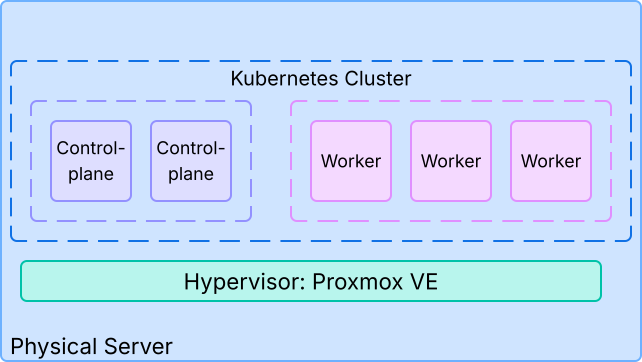
\includegraphics[width=0.7\textwidth]{k8s-cluster}
	\caption{Kubernetes cluster με δύο κόμβους επιπέδου ελέγχου και τρεις κόμβους εργασίας}
	\label{fig:k8s-cluster}
\end{figure}

\section{Ροή δεδομένων σε πραγματικό χρόνο}

\subsection{Πηγές ροής δεδομένων}

Η αξιόπιστη και χαμηλής καθυστέρησης επεξεργασία ροών δεδομένων σε περιβάλλοντα
γεωργίας ακρίβειας προϋποθέτει την ύπαρξη ποικίλων, ετερογενών πηγών δεδομένων
που παρέχουν συνεχή και διαχρονικά κρίσιμη πληροφορία σχετικά με τη φυσική
κατάσταση του αγροτεμαχίου και τις περιβαλλοντικές μεταβλητές. Η παρούσα
πλατφόρμα σχεδιάστηκε ώστε να ενσωματώνει και να επεξεργάζεται δεδομένα σε
πραγματικό χρόνο από πηγές δεδομένων όπως αισθητήρες θερμοκρασίας και υγρασίας
εδάφους ή μετρητές βροχόπτωσης και φωτεινότητας.

\subsection{Τεχνολογίες Streaming}

Στην προηγούμενη ενότητα παρουσιάστηκε το \textit{Apache Kafka} ως το βασικό
μέσο ενδιάμεσης επικοινωνίας μεταξύ των στοιχείων της πλατφόρμας. Σενάρια
\textit{streaming}, όπως αυτό της πλατφόρμας \textit{Nostradamus}, βασίζονται
στο \textit{Kafka} ως τον κεντρικό κόμβο του συστήματος, ο οποίος λειτουργεί ως
η κύρια <<πηγή αλήθειας>> για όλα τα υποσυστήματα. Κάθε γεγονός που συμβαίνει
στο σύστημα καταγράφεται αρχικά στο \textit{Kafka}, και στη συνέχεια κάθε
μικροϋπηρεσία εγγράφεται στο αντίστοιχο <<θέμα>> (\textit{topic}) ώστε να
λαμβάνει μόνο τα μηνύματα που της είναι απαραίτητα. Με αυτόν τον τρόπο
επιτυγχάνεται ο σαφής διαχωρισμός ανάμεσα στη ροή δεδομένων σε πραγματικό χρόνο
και στην κατανάλωση των μηνυμάτων. Συνεπώς, η σωστή σχεδίαση της υποδομής
συλλογής και μεταφοράς δεδομένων έως το \textit{Kafka} είναι κρίσιμη, καθώς από
εκεί και πέρα ο διαμοιρασμός τους στα υπόλοιπα υποσυστήματα γίνεται με απλό και
αποδοτικό τρόπο.

Για το \textit{deployment} του \textit{Kafka} στην πλατφόρμα επιλέχθηκε το
μοτίβο του \textit{Kubernetes Operator}, με στόχο την υψηλή διαθεσιμότητα, την
ανθεκτικότητα σε αστοχίες και την αυτοματοποιημένη διαχείριση του κύκλου ζωής
του συστήματος. Συγκεκριμένα, χρησιμοποιήθηκε ο \textit{Strimzi Kafka
	Operator}, ο οποίος παρέχει πλήρη αυτοματοποίηση στην εγκατάσταση, ρύθμιση,
κλιμάκωση και αναβάθμιση των brokers, καθώς και στη διαχείριση των
\textit{topics} και των \textit{users}. Με αυτόν τον τρόπο αξιοποιούνται τα
πλεονεκτήματα του Kubernetes, όπως η ευκολία κλιμάκωσης, η αυτόματη
αποκατάσταση υπηρεσιών και η συνεπής διαχείριση πόρων, εξασφαλίζοντας παράλληλα
σταθερή και αποδοτική λειτουργία της υποδομής ροών. Τέλος, ο \textit{operator}
αυτός επιτρέπει την διαχείριση της υποδομής του \textit{Kafka} μέσω
\textit{GitOps} πρακτικών, γεγονός που ευθυγραμμίζεται με τις υπόλοιπες αρχές
και πρότυπα σχεδίασης της παρούσας εργασίας.

Είναι πλέον καθιερωμένη πρακτική οι αισθητήρες και γενικότερα οι χαμηλής
κατανάλωσης μικροελεγκτές που χρησιμοποιούνται σε υποδομές \textit{IoT} να
αποστέλλουν τα μηνύματά τους μέσω του πρωτοκόλλου \textit{MQTT}, καθώς αυτό
εξοικονομεί ενέργεια και επιτρέπει αποδοτική μετάδοση δεδομένων. Για την
εισαγωγή των μηνυμάτων αυτής της μορφής στο \textit{Kafka} απαιτείται η ύπαρξη
μηχανισμού γεφύρωσης. Στο πλαίσιο αυτό, αξιοποιήθηκε αρχικά το \textit{Strimzi
	MQTT bridge}.

Ωστόσο, η ενσωματωμένη υλοποίηση του \textit{Strimzi} δεν υποστηρίζει ασφαλή
μεταφορά μέσω \textit{MQTTs}, γεγονός που αποτελεί κρίσιμο ζήτημα για την
παρούσα πλατφόρμα, δεδομένου ότι οι αισθητήρες βρίσκονται σε εξωτερικά δίκτυα.
Για την επίλυση του προβλήματος, ενσωματώθηκε ένας \textit{EMQX broker}, ο
οποίος λειτουργεί ως ασφαλής πύλη (\textit{secure gateway}) μεταξύ των
εξωτερικών συσκευών και του \textit{Kafka}, παρέχοντας υποστήριξη για
κρυπτογράφηση και μηχανισμούς πιστοποίησης σύμφωνα με τις απαιτήσεις της
αρχιτεκτονικής. Παράλληλα, ο \textit{EMQX broker} παρέχει δυνατότητες
φιλτραρίσματος βάσει των εισερχόμενων \textit{MQTT topics} και αντιστοίχισης
(\textit{mapping}) αυτών σε \textit{Kafka topics}, ώστε να προωθούνται στο
\textit{Kafka} μόνο τα απαραίτητα μηνύματα και να διατηρείται συνεπής η
ονοματολογία και η δομή των θεμάτων στην πλατφόρμα.

\subsection{Παρατηρησιμότητα Streaming}

Η παρατηρησιμότητα σε περιβάλλοντα επεξεργασίας ροών δεδομένων αποτελεί
καθοριστικό παράγοντα για την αξιοπιστία και την έγκαιρη λήψη αποφάσεων. Σε
ένα αγροτικό οικοσύστημα, η καθυστέρηση στην ανίχνευση αποτυχίας ή
απώλειας δεδομένων μπορεί να οδηγήσει σε εσφαλμένες εκτιμήσεις για την
κατάσταση του χωραφιού, επηρεάζοντας αρνητικά την παραγωγή. Για τον λόγο
αυτό, η πλατφόρμα \textit{Nostradamus} ενσωματώνει μηχανισμούς
παρατηρησιμότητας που καλύπτουν όλα τα στάδια της ροής δεδομένων, από τη
λήψη μηνυμάτων σε επίπεδο αισθητήρα έως την κατανάλωσή τους από τις
εφαρμογές ανάλυσης.

Στο επίπεδο του \textit{Apache Kafka}, κρίσιμη σημασία έχουν οι μετρικές που
σχετίζονται με τον ρυθμό παραγωγής και κατανάλωσης μηνυμάτων, την καθυστέρηση
στην επεξεργασία (\textit{consumer lag}) και τη χρήση των πόρων του συστήματος
(π.χ. μνήμη, αποθηκευτικός χώρος και δίκτυο). Οι μετρικές αυτές συλλέγονται
αυτόματα μέσω του \textit{Prometheus}, ο οποίος αντλεί δεδομένα από τους
\textit{exporters} του Kafka και του \textit{Strimzi Operator}. Στη συνέχεια,
προβάλλονται σε εξατομικευμένους πίνακες ελέγχου (\textit{dashboards}) στο
\textit{Grafana}, παρέχοντας στους διαχειριστές μια ολοκληρωμένη εικόνα της
κατάστασης του συστήματος σε πραγματικό χρόνο.

Εκτός από τις μετρικές, σημαντική είναι και η ιχνηλασιμότητα (\textit{tracing})
των γεγονότων. Η υιοθέτηση εργαλείων όπως το \textit{OpenTelemetry} σε
συνδυασμό με το \textit{Jaeger} παρέχει τη δυνατότητα για παρακολούθηση του
μονοπατιού ενός μηνύματος σε όλο τον κύκλο ζωής του, από την είσοδό του στον
\textit{EMQX broker} και τη δρομολόγησή του στο \textit{Kafka}, έως και την
κατανάλωσή του από μια υπηρεσία ανάλυσης. Με τον τρόπο αυτό, καθίσταται ,
θεωρητικά, εφικτός ο εντοπισμός καθυστερήσεων ή σημείων συμφόρησης
(\textit{bottlenecks}), γεγονός που επιτρέπει την έγκαιρη διάγνωση και
αντιμετώπισή τους.

Τέλος, μπορούν να οριστούν κανόνες ειδοποίησης (\textit{alerting rules}) στο
\textit{Prometheus}, οι οποίοι θα ενεργοποιούν ειδοποιήσεις σε περίπτωση
ανωμαλιών, όπως υπερβολική καθυστέρηση κατανάλωσης ή απώλεια επικοινωνίας με
κάποιον broker. Οι ειδοποιήσεις αυτές, μέσω του \textit{Alertmanager}, είναι
δυνατόν να προωθούνται σε κανάλια επικοινωνίας (π.χ. ηλεκτρονικό ταχυδρομείο ή
chatops εργαλεία), ώστε οι χειριστές του συστήματος να ενημερώνονται άμεσα για
κρίσιμα περιστατικά.

Συνολικά, η παρατηρησιμότητα της ροής δεδομένων δεν περιορίζεται απλώς στη
συλλογή μετρήσεων, αλλά συνιστά μια ενιαία προσέγγιση που συνδυάζει μετρικές,
ιχνηλασιμότητα και ειδοποιήσεις, επιτρέποντας στην πλατφόρμα να διατηρεί υψηλά
επίπεδα αξιοπιστίας και διαθεσιμότητας σε περιβάλλοντα γεωργίας ακρίβειας.

\subsection{Ανθεκτικότητα και ανοχή σε σφάλματα}

Η πλατφόρμα \textit{Nostradamus} σχεδιάστηκε με γνώμονα την αποφυγή ενιαίων
σημείων αστοχίας και την προβλέψιμη αποκατάσταση υπηρεσιών. Σε επίπεδο
\textit{Kubernetes}, η απομόνωση του \textit{control plane} από τους
\textit{workers} διασφαλίζει ότι αστάθειες εφαρμογών δεν επηρεάζουν τον
συντονισμό του \textit{cluster}. O \textit{scheduler} σε συνδυασμό με
\textit{PodDisruptionBudgets} και \textit{anti-affinity rules} κατανέμουν
φορτία, ενώ τα \textit{liveness/readiness probes} παρέχουν ταχεία ανίχνευση
αστοχιών και επανεκκίνηση \textit{pods}.

Στο επίπεδο μηνυμάτων, το \textit{Apache Kafka} (μέσω \textit{Strimzi})
αξιοποιεί αντιγραφή τμημάτων (\textit{partitions}) με ρυθμίσιμους συντελεστές
πλεονασμού και πολιτικές \textit{acknowledgements}, ώστε απώλειες κόμβων να μην
συνεπάγονται απώλεια δεδομένων. Η μέτρηση \textit{consumer lag}, λόγου χάριν,
αποτελεί πρώιμο δείκτη συμφόρησης ή σιωπηλής αποτυχίας καταναλωτή. Για την
πλευρά αποθήκευσης, το \textit{persistence} υλοποιείται σε \textit{ScyllaDB} με
συνδιαμόρφωση αντιγραφής και ανεκτικότητας σε αστοχίες κόμβων.

Το υποσύστημα ειδοποιήσεων (\textit{Prometheus} + \textit{Alertmanager})
ενεργοποιεί κανόνες για κρίσιμες ανωμαλίες (π.χ. υπέρβαση ορίων \textit{lag},
μη διαθεσιμότητα brokers, μη προσβάσιμες υπηρεσίες). Η αποκατάσταση γίνεται
κατά προτεραιότητα με αυτοματισμούς σε επίπεδο \textit{Kubernetes}
(επανεκκίνηση, \textit{rescheduling}) και, όπου απαιτείται, με ελαφρές
παρεμβάσεις λειτουργικής βελτίωσης (π.χ. ρύθμιση ρυθμού κατανάλωσης ή διάθεση
περισσότερων πόρων σε συγκεκριμένα pods).

Συνολικά, η ανθεκτικότητα προκύπτει από:

\begin{enumerate}
	\item Απομόνωση ρόλων κόμβων
	\item Οριζόντια κλιμάκωση και αντιγραφές
	\item Συνεχή παρακολούθηση και έγκαιρη ειδοποίηση
	\item Προβλέψιμες διαδικασίες ανάκαμψης που ελαχιστοποιούν τον χρόνο μη διαθεσιμότητας.
\end{enumerate}

\section{Υπηρεσίες Εφαρμογών}

\subsection{API εξυπηρέτησης δεδομένων}

Για την κατανάλωση των δεδομένων από τα downstream συστήματα και την
παροχή τους σε εφαρμογές οπτικοποίησης, αναπτύχθηκε μια υπηρεσία API
στη γλώσσα \textit{Go}. Το API προσφέρει REST endpoints για υγεία
συστήματος (\texttt{/healthz}), μετρικές παρακολούθησης (\texttt{/metrics}),
καθώς και αναζήτηση πρόσφατων μετρήσεων αισθητήρων (\texttt{/latest}).

Η αρχιτεκτονική ακολουθεί modular σχεδίαση, με διακριτά πακέτα για
πρόσβαση στη βάση δεδομένων, διαχείριση cache, δρομολόγηση αιτημάτων
και βοηθητικές λειτουργίες. Η επικοινωνία με τη ScyllaDB υλοποιείται
μέσω του οδηγού \texttt{gocql}, ενώ για την κρυφή μνήμη
χρησιμοποιείται το \texttt{go-redis} client.

Για την αποφυγή καθυστερήσεων, κάθε αίτημα προς το API εκτελείται αρχικά με
αναζήτηση στην κρυφή μνήμη (Valkey). Σε περίπτωση αποτυχίας ή ελλιπών
αποτελεσμάτων, το API προσφεύγει στη ScyllaDB και παράλληλα ενημερώνει εκ νέου
την cache. Με αυτόν τον τρόπο εξασφαλίζεται χαμηλή καθυστέρηση για συχνά
αιτήματα, ενώ η ScyllaDB παραμένει η πηγή αλήθειας (\textit{source of truth})
για τα δεδομένα.

\subsubsection{Στρατηγικές caching}

Η υιοθέτηση μηχανισμών κρυφής μνήμης σε κατανεμημένα συστήματα συνοδεύεται από
διαφορετικά πρότυπα (\textit{patterns}) υλοποίησης, καθένα από τα οποία φέρει
πλεονεκτήματα και περιορισμούς. Τα συνηθέστερα είναι τα ακόλουθα:

\paragraph{Read-through}

Στο πρότυπο αυτό, όλες οι αναγνώσεις δεδομένων
γίνονται μέσω της cache. Σε περίπτωση που το ζητούμενο κλειδί δεν υπάρχει, η
ίδια η cache αναλαμβάνει να ανακτήσει τα δεδομένα από τη βάση και να τα
αποθηκεύσει πριν τα επιστρέψει στον χρήστη. Το πλεονέκτημα είναι η απλοποίηση
της εφαρμογής, καθώς η λογική ανάκτησης μετατίθεται στο cache layer. Ωστόσο,
απαιτείται στενή ενσωμάτωση της cache με τη βάση, κάτι που δυσχεραίνει την
παραμετροποίηση σε περιβάλλοντα με ετερογενείς πηγές δεδομένων.

\paragraph{Write-through}

Σε αυτήν τη στρατηγική, κάθε εγγραφή περνάει πρώτα
από την cache και στη συνέχεια στη βάση δεδομένων. Η μέθοδος αυτή εξασφαλίζει
συνεπή δεδομένα, καθώς cache και βάση ενημερώνονται ταυτόχρονα, αλλά αυξάνει
τον χρόνο απόκρισης για κάθε write. Επιπλέον, το συνολικό throughput
περιορίζεται από τον πιο αδύναμο (αργό) κρίκο της αλυσίδας.

\paragraph{Write-behind (ή Write-back)}

Τα δεδομένα γράφονται αρχικά μόνο στην
cache και σε δεύτερο χρόνο, με ασύγχρονο τρόπο, προωθούνται στη βάση. Το σχήμα
αυτό προσφέρει υψηλές επιδόσεις για σενάρια έντονου write load, αλλά εισάγει
κινδύνους απώλειας δεδομένων σε περίπτωση αστοχίας της cache, ενώ η βάση
ενδέχεται να μην αντικατοπτρίζει την πιο πρόσφατη κατάσταση.

\paragraph{Cache-aside (ή Lazy loading)}

Στο πρότυπο αυτό, η εφαρμογή ελέγχει πρώτα την cache. Αν τα δεδομένα υπάρχουν,
επιστρέφονται άμεσα. Αν όχι, η εφαρμογή ανατρέχει στη βάση δεδομένων,
επιστρέφει τα αποτελέσματα στον χρήστη και ταυτόχρονα τα εισάγει εκ νέου στην
cache για μελλοντική χρήση. Το κύριο πλεονέκτημα είναι η απλότητα: η cache
λειτουργεί ως προαιρετικό επιταχυντικό στρώμα, χωρίς να απαιτείται βαθιά
ενσωμάτωση με τη βάση δεδομένων. Το μειονέκτημα είναι ότι τα δεδομένα μπορεί να
είναι στιγμιαία \textit{stale}, ειδικά σε περιπτώσεις έντονων ενημερώσεων.

\medskip Για τις ανάγκες της παρούσας πλατφόρμας, επιλέχθηκε το πρότυπο
\textit{cache-aside}, καθώς τα ερωτήματα αφορούν κυρίως αναγνώσεις πρόσφατων
τιμών αισθητήρων με χαμηλή πιθανότητα συνεχών τροποποιήσεων. Με τον τρόπο αυτό,
η ScyllaDB παραμένει η πηγή αλήθειας (\textit{source of truth}), ενώ το Valkey
cluster χρησιμοποιείται για να μειώσει τον χρόνο απόκρισης σε συχνά αιτήματα,
επιτυγχάνοντας ισορροπία ανάμεσα σε απόδοση και συνέπεια.

\begin{figure}[H]
	\centering
	\includegraphics[width=0.7\textwidth]{cache-aside}
	\caption{Λογικό διάγραμμα του προτύπου \textit{cache-aside}:
		το API ελέγχει αρχικά την κρυφή μνήμη (Valkey) για την αναζήτηση
		δεδομένων και, σε περίπτωση αποτυχίας, προσφεύγει στη ScyllaDB.
		Τα δεδομένα επιστρέφονται στον χρήστη και ταυτόχρονα επανεισάγονται
		στην cache, ώστε να εξυπηρετηθούν με χαμηλή καθυστέρηση σε επόμενα
		αιτήματα.}
	\label{fig:cache-aside-diagram}
\end{figure}

\subsection{Valkey cluster}

Η υποστήριξη του μηχανισμού cache υλοποιείται με \textit{Valkey cluster},
ο οποίος αναπτύχθηκε μέσω του \textit{Hyperspike Operator}. Η λύση αυτή
εξασφαλίζει οριζόντια κλιμάκωση και υψηλή διαθεσιμότητα σε περιβάλλον
Kubernetes, με αυτοματοποιημένη διαχείριση των κόμβων Redis/Valkey.

Συνδυάζοντας τον Valkey cluster για ταχύτατη εξυπηρέτηση πρόσφατων
μετρήσεων με τη ScyllaDB για ανθεκτική και αναλυτική αποθήκευση, η
πλατφόρμα διατηρεί ισορροπία ανάμεσα σε χαμηλή καθυστέρηση και
αξιοπιστία δεδομένων.

\section{Ένταξη πελάτη}

\begin{figure}[H]
	\centering
	\includegraphics[width=0.7\textwidth]{client-onboarding-process}
	\caption{Διάγραμα δραστηριότητας για τη διαδικασία ένταξης νέου πελάτη}
	\label{fig:client-onboarding-activity}
\end{figure}
